% !Mode:: "TeX:UTF-8"
\chapter{模型预测结果的分析与比较}
\label{chap:theory}

\section{模型自分析与结果展示}

本文在评价模型求解的4种方法时,采用了PCC和RMSE作为评价指标:

\begin{equation*}
\mathrm{PCC} = \frac{\sum_{i=1}^{N}(x_i-\overline{x})(y_i-\overline{y})}{\sqrt{\sum_{i=1}^{N}(x_i-\overline{x})^2\sum_{i=1}^{N}(y_i-\overline{y})^2}},
\end{equation*}

\begin{equation*}
\mathrm{RMSE} = \sqrt{\frac{1}{N} \sum_{i=1}^{N} (y_i - x_i)^2}.
\end{equation*}

本文首先在O'Neil数据集上使用4种不同方法对模型的超参数进行求解,从时间成本的角度考虑,基于利用32核CPU进行多进程运算的情况,比较不同方法的时间成本。结果显示,精细调参法的时间成本最高,需要耗费6小时的时间。其次是邻居数统一法,虽然相对较高,但仍需3小时。而邻居数和衰减率统一法的时间成本较小,仅需1小时多。最后,药物组合相似性阈值法的时间成本最低,仅需半小时完成运算。因此,仅就时间成本而言,药物组合相似性阈值法是最优选择。

\begin{table}[htbp]
  \centering
  \caption{DCSN模型不同求解方法的评价指标}
  \label{table:model-4m}
  \small
  \begin{tabular}{p{5cm}cc}
    \toprule
    方法 & PCC & RMSE \\
    \midrule
    精细调参法 & 0.675 & 0.794 \\
    邻居数统一法 & 0.612 & 0.820 \\
    邻居数和衰减率统一法 & 0.611 & 0.820 \\
    药物组合相似性阈值法 & 0.593 & 0.831 \\
    \bottomrule
  \end{tabular}
\end{table}

通过对比分析表\ref{table:model-4m}中不同方法的评价指标,可以发现在O'Neil数据集上,精细调参法得到的结果是最优的。在PCC这一指标上,该方法达到了约0.675的最高水平,而RMSE值则降低至约0.794的最低水平。相比之下,药物组合相似性阈值法的PCC最低,而邻居数统一法与邻居数和衰减率统一法的PCC显著低于精细调参法。药物组合相似性阈值法的PCC之所以较低,是因为在实验过程中,某些目标药物组合存在高相似的邻居但整体的相似性不是很高,当药物组合相似性阈值设定超过0.597时,超过该阈值的邻居药物组合数量变为零,因此无法继续寻找目标药物组合的更高相似邻居,此时该方法设定的相似性阈值所得到的结果即为其能够找到的最优结果。

\newpage % 强制换页

\begin{center} % 表格居中显示
\small % 缩小字号
\renewcommand{\arraystretch}{0.6} % 设置行高
\begin{longtable}{@{}lcccc@{}} % 设置表格列格式,并移除边距
\caption{基于精细调参法求解的部分结果(O'Neil数据集)} \\
\toprule
\textbf{Drug Combination} & \textbf{Neighbors} & \textbf{alp} & \textbf{PCC} & \textbf{RMSE} \\
\midrule
\endfirsthead

\multicolumn{5}{@{}c@{}}%
{{\tablename\ \thetable{} -- 续页}} \\
\toprule
\textbf{Drug Combination} & \textbf{Neighbors} & \textbf{alp} & \textbf{PCC} & \textbf{RMSE} \\
\midrule
\endhead

\midrule
\multicolumn{5}{r}{{Continued on next page}} \\ % 在下一页继续表头
\endfoot

\bottomrule
\endlastfoot

    'MK-5108', 'SORAFENIB' & 43 & 3.00 & 0.80 & 0.69 \\
    'VINORELBINE', 'SUNITINIB' & 16 & 3.00 & 0.67 & 0.78 \\
    'SUNITINIB', 'MK-8776' & 46 & 3.00 & 0.75 & 0.74 \\
    '5-FU', 'DINACICLIB' & 7 & 3.00 & 0.41 & 0.92 \\
    'SUNITINIB', 'MK-2206' & 52 & 3.00 & 0.62 & 0.83 \\
    'PACLITAXEL', 'BEZ-235' & 4 & 3.00 & 0.90 & 0.49 \\
    'MK-2206', 'DINACICLIB' & 48 & 3.00 & 0.48 & 0.91 \\
    'MK-4827', 'MK-8776' & 54 & 3.00 & 0.70 & 0.79 \\
    'VINORELBINE', 'DINACICLIB' & 25 & 3.00 & 0.35 & 0.94 \\
    'MK-5108', 'MK-8776' & 2 & 3.00 & 0.82 & 0.57 \\
    'TEMOZOLOMIDE', 'SN-38' & 58 & 3.00 & 0.78 & 0.79 \\
    'ETOPOSIDE', 'MK-8669' & 65 & 3.00 & 0.79 & 0.76 \\
    'SUNITINIB', 'MK-4827' & 47 & 3.00 & 0.67 & 0.81 \\
    'BORTEZOMIB', 'GELDANAMYCIN' & 78 & 3.00 & 0.81 & 0.76 \\
    'PACLITAXEL', 'ABT-888' & 27 & 3.00 & 0.83 & 0.70 \\
    'CYCLOPHOSPHAMIDE', 'BEZ-235' & 44 & 3.00 & 0.86 & 0.70 \\
    'DASATINIB', 'DINACICLIB' & 51 & 3.00 & 0.78 & 0.74 \\
    'METHOTREXATE', 'ERLOTINIB' & 2 & 1.00 & 0.75 & 0.67 \\
    'MK-2206', 'TOPOTECAN' & 72 & 3.00 & 0.65 & 0.84 \\
    'AZD1775', 'MK-4827' & 56 & 3.00 & 0.61 & 0.82 \\
    'METFORMIN', 'BEZ-235' & 62 & 3.00 & 0.89 & 0.61 \\
    'ZOLINZA', 'AZD1775' & 45 & 3.00 & 0.84 & 0.66 \\
    'DASATINIB', 'SORAFENIB' & 2 & 1.00 & 0.61 & 0.79 \\
    'CYCLOPHOSPHAMIDE', 'TEMOZOLOMIDE' & 21 & 3.00 & 0.57 & 0.84 \\
    'MRK-003', 'PACLITAXEL' & 28 & 3.00 & 0.77 & 0.74 \\
    'DEXAMETHASONE', 'LAPATINIB' & 40 & 3.00 & 0.78 & 0.72 \\
    'DEXAMETHASONE', 'MK-8669' & 43 & 3.00 & 0.69 & 0.80 \\
    'ERLOTINIB', 'BEZ-235' & 56 & 3.00 & 0.77 & 0.75 \\
    'VINBLASTINE', 'PD325901' & 83 & 3.00 & 0.55 & 0.88 \\
    'MK-4541', 'METFORMIN' & 51 & 3.00 & 0.71 & 0.80 \\
    'VINORELBINE', 'DASATINIB' & 12 & 3.00 & 0.85 & 0.62 \\
    'METHOTREXATE', 'BORTEZOMIB' & 22 & 3.00 & 0.83 & 0.69 \\
    'GELDANAMYCIN', 'SN-38' & 19 & 3.00 & 0.39 & 0.92 \\
    'ERLOTINIB', 'MK-8669' & 67 & 3.00 & 0.24 & 0.97 \\
    'ABT-888', 'SN-38' & 3 & 1.00 & 0.29 & 1.02 \\
    'MK-4541', 'ETOPOSIDE' & 57 & 3.00 & 0.62 & 0.82 \\
    'CARBOPLATIN', 'DINACICLIB' & 28 & 3.00 & 0.81 & 0.73 \\
    'PD325901', 'SORAFENIB' & 62 & 3.00 & 0.69 & 0.81 \\
    'VINBLASTINE', 'MK-4827' & 62 & 3.00 & 0.71 & 0.80 \\
    'MITOMYCINE', 'MK-2206' & 30 & 3.00 & 0.63 & 0.82 \\
    'MK-4541', 'GELDANAMYCIN' & 61 & 3.00 & 0.66 & 0.83 \\
    'VINBLASTINE', 'AZD1775' & 17 & 3.00 & 0.85 & 0.62 \\
    'SORAFENIB', 'MK-8776' & 16 & 3.00 & 0.71 & 0.74 \\
    'MK-4827', 'DASATINIB' & 2 & 3.00 & 0.86 & 0.52 \\
    'MITOMYCINE', 'TEMOZOLOMIDE' & 32 & 3.00 & 0.61 & 0.81 \\
    'BORTEZOMIB', 'OXALIPLATIN' & 69 & 3.00 & 0.84 & 0.71 \\
    'ERLOTINIB', 'GELDANAMYCIN' & 43 & 3.00 & 0.55 & 0.88 \\
    'MK-5108', 'DINACICLIB' & 2 & 1.00 & 0.68 & 0.74 \\
    'METHOTREXATE', 'TEMOZOLOMIDE' & 25 & 3.00 & 0.73 & 0.73 \\
    'DOXORUBICIN', 'BORTEZOMIB' & 34 & 3.00 & 0.38 & 0.92 \\
    'MITOMYCINE', 'LAPATINIB' & 63 & 3.00 & 0.63 & 0.84 \\
    'L778123', 'SUNITINIB' & 58 & 3.00 & 0.76 & 0.77 \\
    'L778123', 'MK-4827' & 48 & 3.00 & 0.65 & 0.83 \\
    'SN-38', 'SORAFENIB' & 48 & 3.00 & 0.74 & 0.78 \\
    'ZOLINZA', 'SN-38' & 44 & 3.00 & 0.83 & 0.73 \\
    % 'METFORMIN', 'MK-8776' & 25 & 3.00 & 0.53 & 0.86 \\
    % 'ZOLINZA', 'GELDANAMYCIN' & 70 & 3.00 & 0.74 & 0.82 \\
    % 'CYCLOPHOSPHAMIDE', 'SORAFENIB' & 12 & 3.00 & 0.78 & 0.73 \\
    % 'MK-4541', 'L778123' & 59 & 3.00 & 0.63 & 0.83 \\
    % 'ERLOTINIB', 'BORTEZOMIB' & 55 & 3.00 & 0.82 & 0.76 \\
    % 'VINORELBINE', 'MK-5108' & 22 & 3.00 & 0.43 & 0.91 \\
    % 'MK-4541', 'MK-5108' & 44 & 3.00 & 0.54 & 0.86 \\
\end{longtable}
\end{center}

\newpage % 强制换页

\begin{center} % 表格居中显示
\small % 缩小字号
\renewcommand{\arraystretch}{0.6} % 设置行高
\begin{longtable}{@{}lcccc@{}} % 设置表格列格式,并移除边距
\caption{基于邻居数统一法求解的部分结果(O'Neil数据集)} \\
\toprule
\textbf{Drug Combination} & \textbf{Neighbors} & \textbf{alp} & \textbf{PCC} & \textbf{RMSE} \\
\midrule
\endfirsthead

\multicolumn{5}{@{}c@{}}%
{{\tablename\ \thetable{} -- 续页}} \\
\toprule
\textbf{Drug Combination} & \textbf{Neighbors} & \textbf{alp} & \textbf{PCC} & \textbf{RMSE} \\
\midrule
\endhead

\midrule
\multicolumn{5}{r}{{Continued on next page}} \\ % 在下一页继续表头
\endfoot

\bottomrule
\endlastfoot
    'MK-5108', 'SORAFENIB' & 51 & 1.59 & 0.76 & 0.72 \\
    'VINORELBINE', 'SUNITINIB' & 51 & 1.00 & 0.64 & 0.81 \\
    'SUNITINIB', 'MK-8776' & 51 & 3.00 & 0.73 & 0.76 \\
    '5-FU', 'DINACICLIB' & 51 & 3.00 & 0.36 & 0.93 \\
    'SUNITINIB', 'MK-2206' & 51 & 3.00 & 0.61 & 0.83 \\
    'PACLITAXEL', 'BEZ-235' & 51 & 1.00 & 0.75 & 0.75 \\
    'MK-2206', 'DINACICLIB' & 51 & 3.00 & 0.47 & 0.91 \\
    'MK-4827', 'MK-8776' & 51 & 1.00 & 0.68 & 0.79 \\
    'VINORELBINE', 'DINACICLIB' & 51 & 3.00 & 0.28 & 0.96 \\
    'MK-5108', 'MK-8776' & 51 & 1.00 & 0.65 & 0.80 \\
    'TEMOZOLOMIDE', 'SN-38' & 51 & 3.00 & 0.75 & 0.80 \\
    'ETOPOSIDE', 'MK-8669' & 51 & 3.00 & 0.75 & 0.76 \\
    'SUNITINIB', 'MK-4827' & 51 & 3.00 & 0.63 & 0.82 \\
    'BORTEZOMIB', 'GELDANAMYCIN' & 51 & 1.00 & 0.78 & 0.76 \\
    'PACLITAXEL', 'ABT-888' & 51 & 1.00 & 0.70 & 0.81 \\
    'CYCLOPHOSPHAMIDE', 'BEZ-235' & 51 & 3.00 & 0.84 & 0.71 \\
    'DASATINIB', 'DINACICLIB' & 51 & 3.00 & 0.78 & 0.74 \\
    'METHOTREXATE', 'ERLOTINIB' & 51 & 1.00 & 0.39 & 0.92 \\
    'MK-2206', 'TOPOTECAN' & 51 & 1.00 & 0.56 & 0.87 \\
    'AZD1775', 'MK-4827' & 51 & 3.00 & 0.59 & 0.82 \\
    'METFORMIN', 'BEZ-235' & 51 & 3.00 & 0.88 & 0.58 \\
    'ZOLINZA', 'AZD1775' & 51 & 3.00 & 0.83 & 0.66 \\
    'DASATINIB', 'SORAFENIB' & 51 & 1.00 & 0.45 & 0.89 \\
    'CYCLOPHOSPHAMIDE', 'TEMOZOLOMIDE' & 51 & 1.00 & 0.40 & 0.92 \\
    'MRK-003', 'PACLITAXEL' & 51 & 1.00 & 0.64 & 0.81 \\
    'DEXAMETHASONE', 'LAPATINIB' & 51 & 3.00 & 0.75 & 0.76 \\
    'DEXAMETHASONE', 'MK-8669' & 51 & 3.00 & 0.68 & 0.81 \\
    'ERLOTINIB', 'BEZ-235' & 51 & 3.00 & 0.74 & 0.76 \\
    'VINBLASTINE', 'PD325901' & 51 & 1.00 & 0.43 & 0.92 \\
    'MK-4541', 'METFORMIN' & 51 & 3.00 & 0.71 & 0.80 \\
    'VINORELBINE', 'DASATINIB' & 51 & 1.00 & 0.78 & 0.71 \\
    'METHOTREXATE', 'BORTEZOMIB' & 51 & 3.00 & 0.78 & 0.72 \\
    'GELDANAMYCIN', 'SN-38' & 51 & 1.00 & 0.31 & 0.95 \\
    'ERLOTINIB', 'MK-8669' & 51 & 3.00 & 0.16 & 1.00 \\
    'ABT-888', 'SN-38' & 51 & 3.00 & 0.22 & 0.98 \\
    'MK-4541', 'ETOPOSIDE' & 51 & 3.00 & 0.60 & 0.83 \\
    'CARBOPLATIN', 'DINACICLIB' & 51 & 1.00 & 0.71 & 0.81 \\
    'PD325901', 'SORAFENIB' & 51 & 3.00 & 0.65 & 0.83 \\
    'VINBLASTINE', 'MK-4827' & 51 & 3.00 & 0.70 & 0.79 \\
    'MITOMYCINE', 'MK-2206' & 51 & 1.00 & 0.56 & 0.86 \\
    'MK-4541', 'GELDANAMYCIN' & 51 & 3.00 & 0.62 & 0.84 \\
    'VINBLASTINE', 'AZD1775' & 51 & 1.00 & 0.77 & 0.73 \\
    'SORAFENIB', 'MK-8776' & 51 & 1.00 & 0.64 & 0.80 \\
    'MK-4827', 'DASATINIB' & 51 & 1.00 & 0.79 & 0.71 \\
    'MITOMYCINE', 'TEMOZOLOMIDE' & 51 & 1.00 & 0.55 & 0.86 \\
    'BORTEZOMIB', 'OXALIPLATIN' & 51 & 1.00 & 0.81 & 0.71 \\
    'ERLOTINIB', 'GELDANAMYCIN' & 51 & 1.00 & 0.45 & 0.91 \\
    'MK-5108', 'DINACICLIB' & 51 & 1.00 & 0.38 & 0.94 \\
    'METHOTREXATE', 'TEMOZOLOMIDE' & 51 & 1.00 & 0.69 & 0.76 \\
    'DOXORUBICIN', 'BORTEZOMIB' & 51 & 3.00 & 0.34 & 0.94 \\
    'MITOMYCINE', 'LAPATINIB' & 51 & 1.00 & 0.59 & 0.85 \\
    'L778123', 'SUNITINIB' & 51 & 3.00 & 0.74 & 0.78 \\
    'L778123', 'MK-4827' & 51 & 1.00 & 0.63 & 0.84 \\
    'SN-38', 'SORAFENIB' & 51 & 3.00 & 0.70 & 0.80 \\
    'ZOLINZA', 'SN-38' & 51 & 1.00 & 0.81 & 0.76 \\
    % 'METFORMIN', 'MK-8776' & 51 & 1.00 & 0.47 & 0.89 \\
    % 'ZOLINZA', 'GELDANAMYCIN' & 51 & 3.00 & 0.69 & 0.84 \\
    % 'CYCLOPHOSPHAMIDE', 'SORAFENIB' & 51 & 1.00 & 0.69 & 0.77 \\
    % 'MK-4541', 'L778123' & 51 & 3.00 & 0.62 & 0.83 \\
    % 'ERLOTINIB', 'BORTEZOMIB' & 51 & 1.00 & 0.80 & 0.76 \\
    % 'VINORELBINE', 'MK-5108' & 51 & 3.00 & 0.37 & 0.93 \\
    % 'MK-4541', 'MK-5108' & 51 & 3.00 & 0.49 & 0.88 \\
    % 'TEMOZOLOMIDE', 'MK-5108' & 51 & 1.00 & 0.79 & 0.72 \\
    % '5-FU', 'ABT-888' & 51 & 3.00 & 0.59 & 0.86 \\
    % 'AZD1775', 'OXALIPLATIN' & 51 & 1.00 & 0.82 & 0.63 \\
    % 'MK-5108', 'MK-2206' & 51 & 3.00 & 0.38 & 0.93 \\
    % 'SUNITINIB', 'GELDANAMYCIN' & 51 & 3.00 & 0.51 & 0.88 \\
    % 'GEMCITABINE', 'LAPATINIB' & 51 & 3.00 & 0.59 & 0.84 \\
\end{longtable}
\end{center}

\newpage % 强制换页

\begin{center} % 表格居中显示
\small % 缩小字号
\renewcommand{\arraystretch}{0.6} % 设置行高
\begin{longtable}{@{}lcccc@{}} % 设置表格列格式,并移除边距
\caption{基于邻居数和衰减率统一法求解的部分结果(O'Neil数据集)} \\
\toprule
\textbf{Drug Combination} & \textbf{Neighbors} & \textbf{alp} & \textbf{PCC} & \textbf{RMSE} \\
\midrule
\endfirsthead

\multicolumn{5}{@{}c@{}}%
{{\tablename\ \thetable{} -- 续页}} \\
\toprule
\textbf{Drug Combination} & \textbf{Neighbors} & \textbf{alp} & \textbf{PCC} & \textbf{RMSE} \\
\midrule
\endhead

\midrule
\multicolumn{5}{r}{{Continued on next page}} \\ % 在下一页继续表头
\endfoot

\bottomrule
\endlastfoot
    'MK-5108', 'SORAFENIB' & 51 & 1.00 & 0.76 & 0.72 \\
    'VINORELBINE', 'SUNITINIB' & 51 & 1.00 & 0.64 & 0.81 \\
    'SUNITINIB', 'MK-8776' & 51 & 1.00 & 0.73 & 0.76 \\
    '5-FU', 'DINACICLIB' & 51 & 1.00 & 0.36 & 0.93 \\
    'SUNITINIB', 'MK-2206' & 51 & 1.00 & 0.61 & 0.83 \\
    'PACLITAXEL', 'BEZ-235' & 51 & 1.00 & 0.75 & 0.75 \\
    'MK-2206', 'DINACICLIB' & 51 & 1.00 & 0.47 & 0.91 \\
    'MK-4827', 'MK-8776' & 51 & 1.00 & 0.68 & 0.79 \\
    'VINORELBINE', 'DINACICLIB' & 51 & 1.00 & 0.28 & 0.96 \\
    'MK-5108', 'MK-8776' & 51 & 1.00 & 0.65 & 0.80 \\
    'TEMOZOLOMIDE', 'SN-38' & 51 & 1.00 & 0.75 & 0.80 \\
    'ETOPOSIDE', 'MK-8669' & 51 & 1.00 & 0.75 & 0.76 \\
    'SUNITINIB', 'MK-4827' & 51 & 1.00 & 0.63 & 0.83 \\
    'BORTEZOMIB', 'GELDANAMYCIN' & 51 & 1.00 & 0.78 & 0.76 \\
    'PACLITAXEL', 'ABT-888' & 51 & 1.00 & 0.70 & 0.81 \\
    'CYCLOPHOSPHAMIDE', 'BEZ-235' & 51 & 1.00 & 0.84 & 0.72 \\
    'DASATINIB', 'DINACICLIB' & 51 & 1.00 & 0.78 & 0.74 \\
    'METHOTREXATE', 'ERLOTINIB' & 51 & 1.00 & 0.39 & 0.92 \\
    'MK-2206', 'TOPOTECAN' & 51 & 1.00 & 0.56 & 0.87 \\
    'AZD1775', 'MK-4827' & 51 & 1.00 & 0.59 & 0.82 \\
    'METFORMIN', 'BEZ-235' & 51 & 1.00 & 0.88 & 0.58 \\
    'ZOLINZA', 'AZD1775' & 51 & 1.00 & 0.83 & 0.66 \\
    'DASATINIB', 'SORAFENIB' & 51 & 1.00 & 0.45 & 0.89 \\
    'CYCLOPHOSPHAMIDE', 'TEMOZOLOMIDE' & 51 & 1.00 & 0.40 & 0.92 \\
    'MRK-003', 'PACLITAXEL' & 51 & 1.00 & 0.64 & 0.81 \\
    'DEXAMETHASONE', 'LAPATINIB' & 51 & 1.00 & 0.75 & 0.76 \\
    'DEXAMETHASONE', 'MK-8669' & 51 & 1.00 & 0.67 & 0.81 \\
    'ERLOTINIB', 'BEZ-235' & 51 & 1.00 & 0.74 & 0.77 \\
    'VINBLASTINE', 'PD325901' & 51 & 1.00 & 0.43 & 0.92 \\
    'MK-4541', 'METFORMIN' & 51 & 1.00 & 0.71 & 0.80 \\
    'VINORELBINE', 'DASATINIB' & 51 & 1.00 & 0.78 & 0.71 \\
    'METHOTREXATE', 'BORTEZOMIB' & 51 & 1.00 & 0.78 & 0.72 \\
    'GELDANAMYCIN', 'SN-38' & 51 & 1.00 & 0.31 & 0.95 \\
    'ERLOTINIB', 'MK-8669' & 51 & 1.00 & 0.16 & 1.00 \\
    'ABT-888', 'SN-38' & 51 & 1.00 & 0.22 & 0.98 \\
    'MK-4541', 'ETOPOSIDE' & 51 & 1.00 & 0.60 & 0.83 \\
    'CARBOPLATIN', 'DINACICLIB' & 51 & 1.00 & 0.71 & 0.81 \\
    'PD325901', 'SORAFENIB' & 51 & 1.00 & 0.65 & 0.83 \\
    'VINBLASTINE', 'MK-4827' & 51 & 1.00 & 0.70 & 0.79 \\
    'MITOMYCINE', 'MK-2206' & 51 & 1.00 & 0.56 & 0.86 \\
    'MK-4541', 'GELDANAMYCIN' & 51 & 1.00 & 0.62 & 0.84 \\
    'VINBLASTINE', 'AZD1775' & 51 & 1.00 & 0.77 & 0.73 \\
    'SORAFENIB', 'MK-8776' & 51 & 1.00 & 0.64 & 0.80 \\
    'MK-4827', 'DASATINIB' & 51 & 1.00 & 0.79 & 0.71 \\
    'MITOMYCINE', 'TEMOZOLOMIDE' & 51 & 1.00 & 0.55 & 0.86 \\
    'BORTEZOMIB', 'OXALIPLATIN' & 51 & 1.00 & 0.81 & 0.71 \\
    'ERLOTINIB', 'GELDANAMYCIN' & 51 & 1.00 & 0.45 & 0.91 \\
    'MK-5108', 'DINACICLIB' & 51 & 1.00 & 0.38 & 0.94 \\
    'METHOTREXATE', 'TEMOZOLOMIDE' & 51 & 1.00 & 0.69 & 0.76 \\
    'DOXORUBICIN', 'BORTEZOMIB' & 51 & 3.00 & 0.34 & 0.94 \\
    'MITOMYCINE', 'LAPATINIB' & 51 & 1.00 & 0.59 & 0.85 \\
    'L778123', 'SUNITINIB' & 51 & 3.00 & 0.74 & 0.78 \\
    'L778123', 'MK-4827' & 51 & 1.00 & 0.63 & 0.84 \\
    'SN-38', 'SORAFENIB' & 51 & 3.00 & 0.70 & 0.80 \\
    'ZOLINZA', 'SN-38' & 51 & 1.00 & 0.81 & 0.76 \\
    % 'METFORMIN', 'MK-8776' & 51 & 1.00 & 0.47 & 0.89 \\
    % 'ZOLINZA', 'GELDANAMYCIN' & 51 & 3.00 & 0.69 & 0.84 \\
    % 'CYCLOPHOSPHAMIDE', 'SORAFENIB' & 51 & 1.00 & 0.69 & 0.77 \\
    % 'MK-4541', 'L778123' & 51 & 3.00 & 0.62 & 0.83 \\
    % 'ERLOTINIB', 'BORTEZOMIB' & 51 & 1.00 & 0.80 & 0.76 \\
\end{longtable}
\end{center}

通过观察各方法的求解结果,可以发现精细调参法中求解的超参数$τ$大多是3或1,大部分是求解区间的端点值。观察到邻居数统一法中求解的超参数$N$集中在51,超参数$τ$大多是3或1,邻居数和衰减率统一法中求解的超参数$N$集中在51,超参数$τ$集中在1。对比邻居数统一法与邻居数和衰减率统一法求解的超参数$τ$和PCC评价指标,可知超参数$τ$对PCC有影响,但影响不大。对比精细调参法和邻居数统一法求解的超参数$N$,对模型影响较大的是超参数$N$。

综合考虑,本文认为精细调参法的超参数求解结果最为优秀。因此,在NCI-ALMANAC数据集上的实验中,本文使用了精细调参法来求解模型。值得注意的是,DCSN模型在两个不同的数据集上都表现出了很高的性能水平,PCC均高于0.670,这表明该模型具有很强的泛化能力,能够适应不同的数据集并取得出色的预测性能。具体来看,模型在两个数据集上的评价指标如表\ref{table:model-mn}所示。

\begin{table}[htbp]
  \centering
  \caption{不同数据集上的模型评价指标}
  \label{table:model-mn}
  \small
  \begin{tabular}{p{5cm}cc}
    \toprule
    数据集 & PCC & RMSE \\
    \midrule
    O'Neil数据集 & 0.675 & 0.794 \\
    NCI-ALMANAC数据集 & 0.684 & 0.719 \\
    \bottomrule
  \end{tabular}
\end{table}

此外,本文绘制了预测协同得分和实际测试值之间的散点图,并采用最小二乘回归法对数据进行拟合,进而求解P值。散点图的绘制有助于评估协同得分和实际测试值之间的关系,通过散点图拟合得到的直线,可以用于预测协同得分和实际测试值之间的关系。P值是用于确定在假设检验中拒绝原假设的概率,常用于确定回归系数是否显著不为零。在回归分析中,如果P值小于0.05,则通常拒绝原假设,认为回归系数显著不为零。因此,基于给定的数据集,通过使用最小二乘回归法对散点图进行拟合,可以得到拟合的直线。接着,可以计算该直线的回归系数和P值,以确定该模型是否显著。如果P值小于0.05,则可认为模型是显著的,可以用该模型预测协同得分和实际测试值之间的关系。

在图\ref{fig:mc}中,使用最小二乘回归法对数据进行拟合,得到了红色直线的函数图。该直线的斜率为0.7065,偏差为$1.387 \times 10^{-10}$,P值计算结果小于0.05,说明回归系数是显著的。在O'Neil数据集上,DCSN的预测结果和实际测试值之间具有很强的线性相关性。而在图\ref{fig:nc}中,可以看到用最小二乘回归法拟合的红色直线,其斜率为1.034,偏差为$-3.578 \times 10^{-18}$。经过P值检验,该回归系数被认为是显著的,P值计算结果小于0.05。在NCI-ALMANAC数据集上,DCSN的预测结果和实际测试值之间具有很强的线性相关性。

\begin{figure}[H]
\centering
  \begin{minipage}{0.45\linewidth}
    \centering
    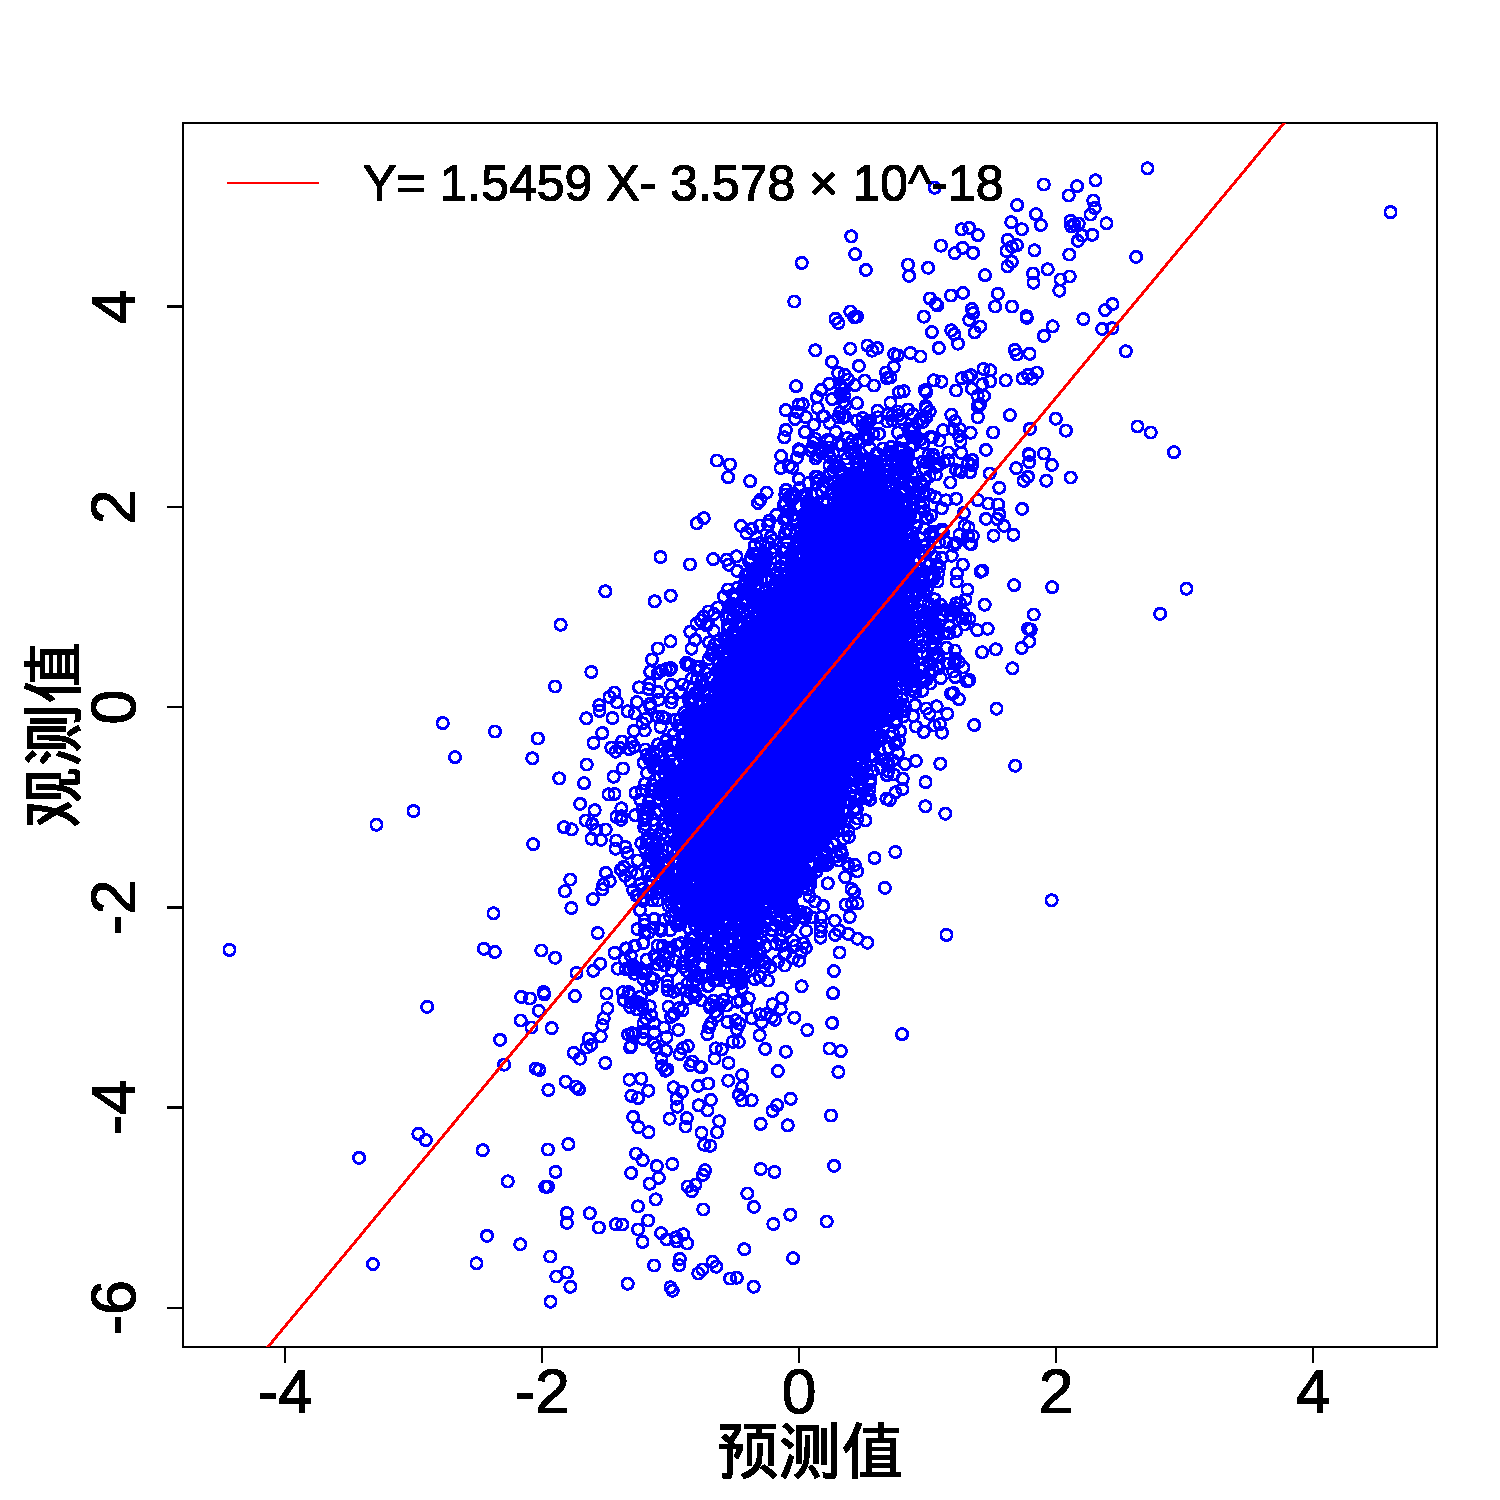
\includegraphics[width=\textwidth]{figures/p_a_scatter_m.pdf}
    \caption{O'Neil数据集的\\预测值和测试值的散点图\label{fig:mc}}
  \end{minipage}
  \begin{minipage}{0.45\linewidth}
    \centering
    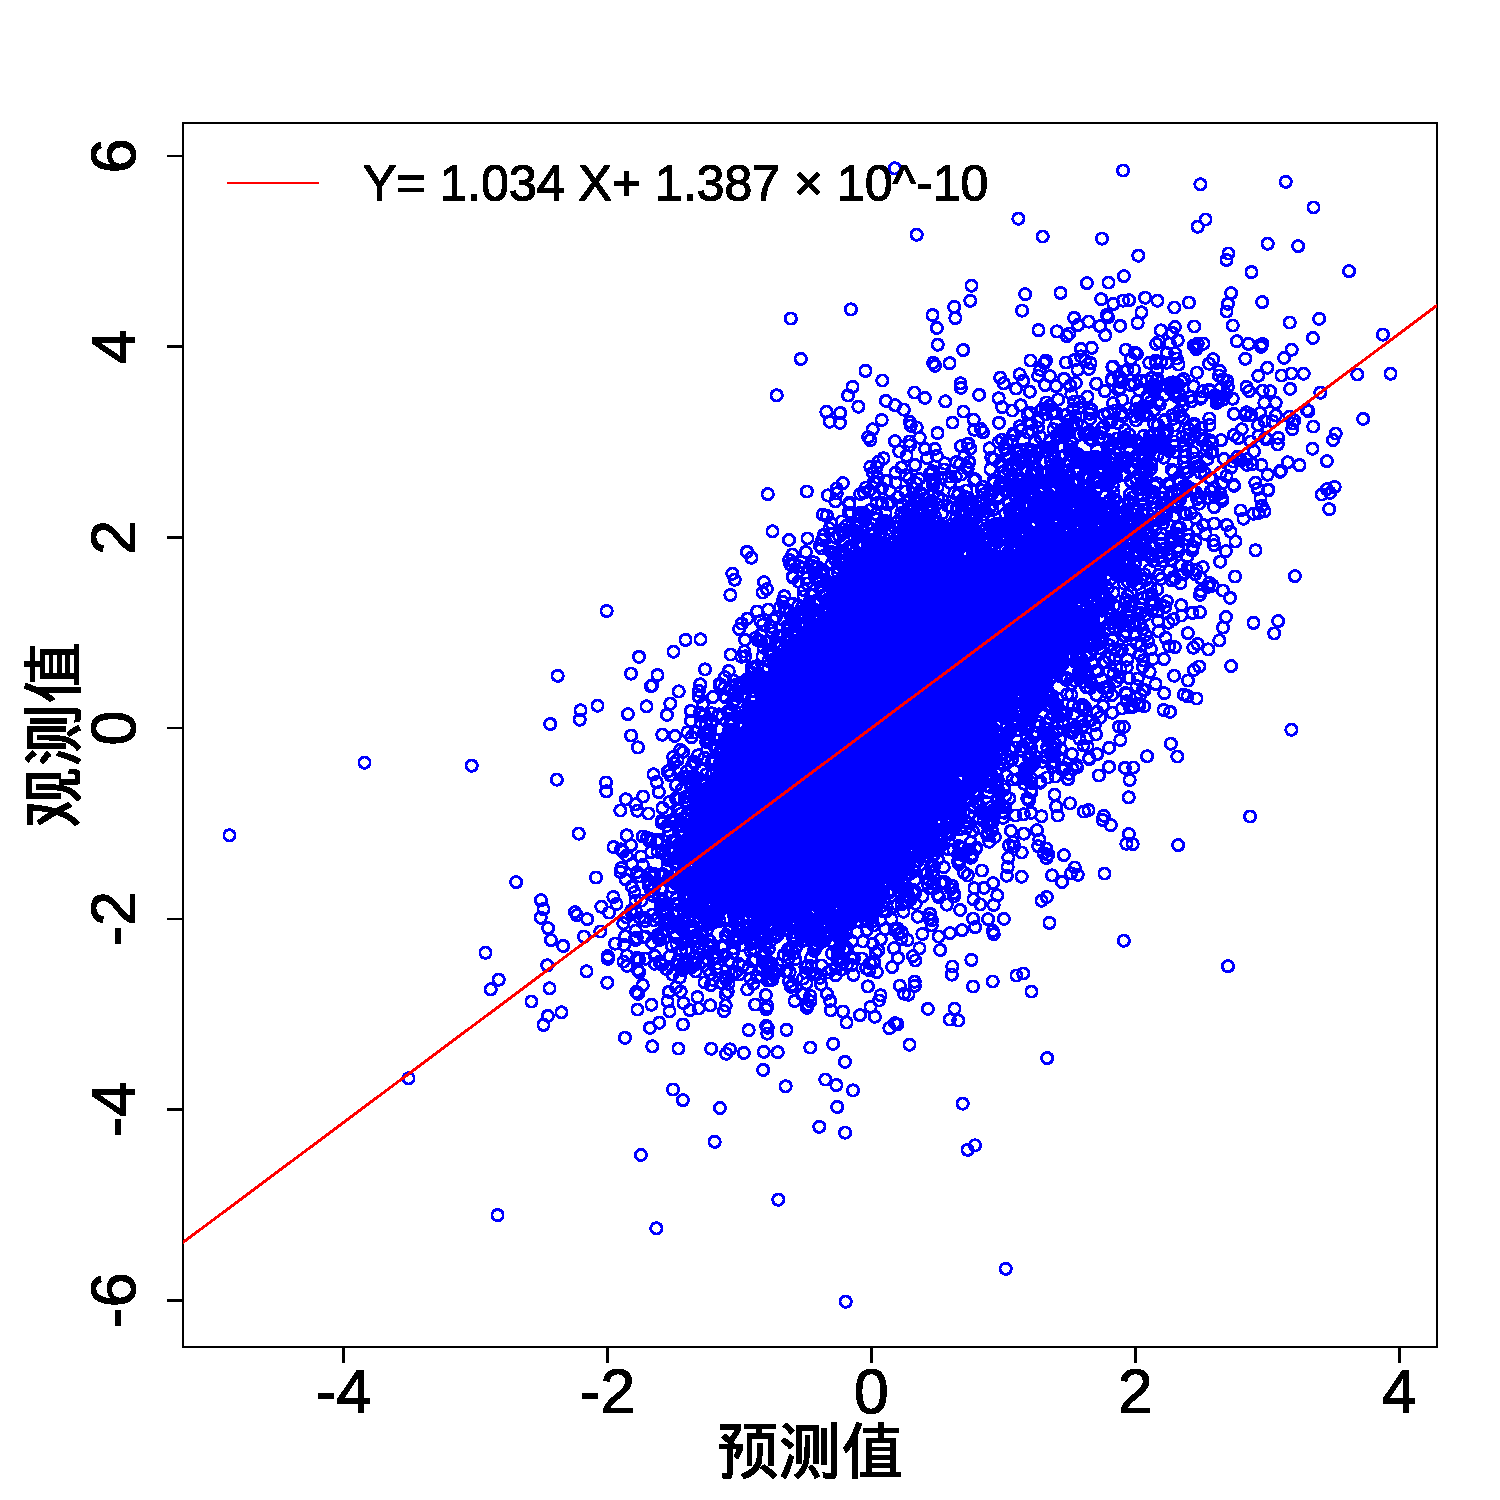
\includegraphics[width=\textwidth]{figures/p_a_scatter.pdf}
    \caption{NCI-ALMANAC数据集的\\预测值和测试值的散点图\label{fig:nc}}
  \end{minipage}
\end{figure}

无论是基于O'Neil数据集还是NCI-ALMANAC数据集,DCSN模型预测结果的拟合函数都表明,DCSN的预测结果和实际测试值之间具有很强的线性相关性。因此,可以得出结论,DCSN模型是一个有效的预测模型,可以用于生物医学领域中的药物组合筛选和发现。

为了统计数据集预测结果中每个药物组合的邻居数情况,本文制作了药物组合邻居数的柱状图,如图\ref{fig:md}和图\ref{fig:nd}所示。其中,可以看到O'Neil数据集中大部分药物组合的高相似邻居数集中在150以前,NCI-ALMANAC数据集中大部分药物组合的高相似邻居数集中在100以前,这说明这些数据集中的药物组合之间的化学结构相似度程度存在差异。

\begin{figure}[H]
\centering
  \begin{minipage}{0.45\linewidth}
    \centering
    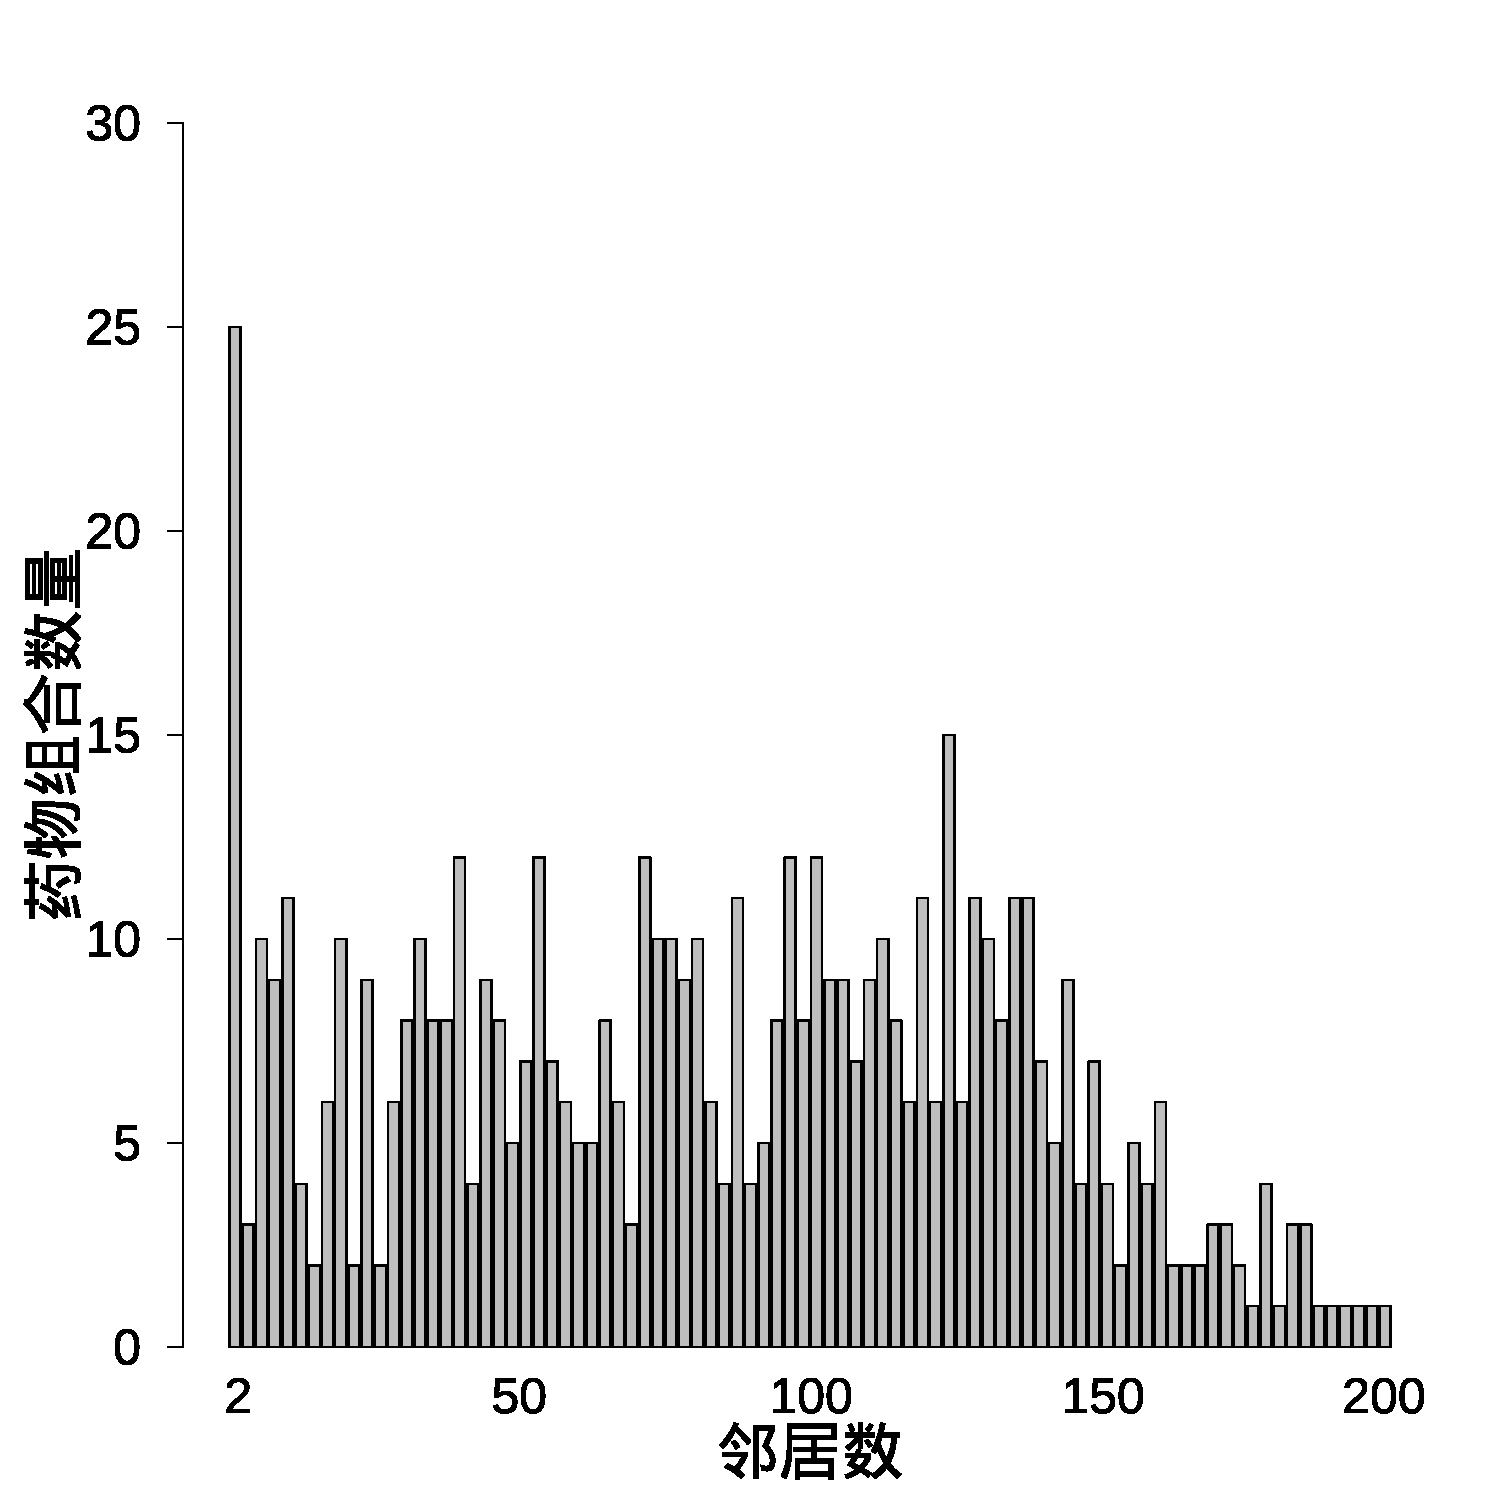
\includegraphics[width=\textwidth]{figures/m_barplot.pdf}
    \caption{基于O'Neil数据集的\\药物组合邻居数柱状图\label{fig:md}}
  \end{minipage}
  \begin{minipage}{0.45\linewidth}
    \centering
    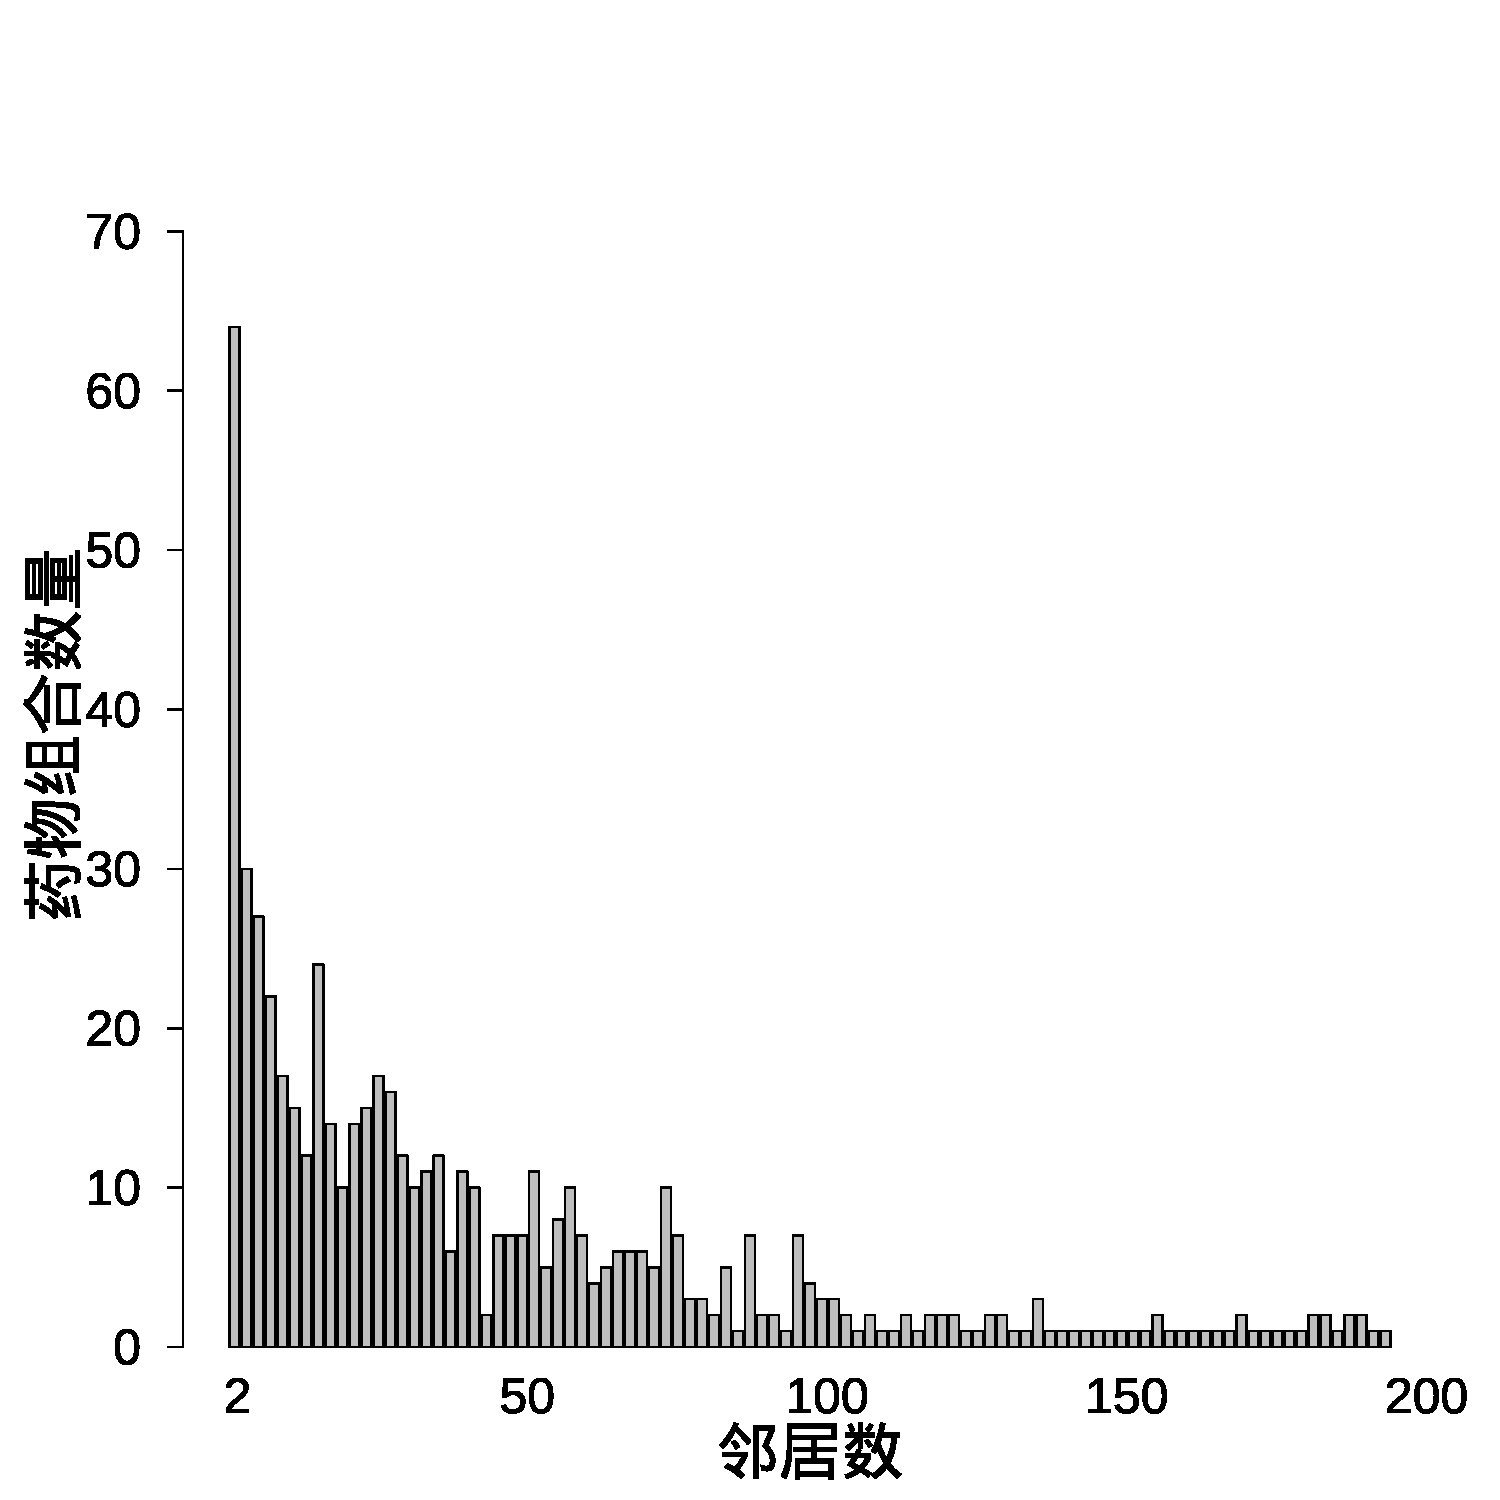
\includegraphics[width=\textwidth]{figures/n_barplot.pdf}
    \caption{基于NCI-ALMANAC数据集的\\药物组合邻居数柱状图\label{fig:nd}}
  \end{minipage}
\end{figure}

\newpage

\begin{figure}[H]
\centering
  \begin{minipage}{0.45\linewidth}
    \centering
    \includegraphics[width=\textwidth]{figures/heatmap_m}
    \caption{基于O'Neil数据集的\\药物组合相似性热图\label{fig:mht}}
  \end{minipage}
  \begin{minipage}{0.45\linewidth}
    \centering
    \includegraphics[width=\textwidth]{figures/heatmap_n}
    \caption{基于NCI-ALMANAC数据集的\\药物组合相似性热图\label{fig:nht}}
  \end{minipage}
\end{figure}

为了探索数据集中的药物组合之间的化学结构相似度的差异程度,本文制作了药物组合相似性热图如图\ref{fig:mht}和图\ref{fig:nht}所示。可以发现后者的红色部分明显比前者多。这一现象说明NCI-ALMANAC数据集中的药物组合之间的化学结构相似度更高,因此使用相对较少的高相似邻居数就足以提供有用的信息,而O'Neil数据集中的药物组合之间的化学结构相似度相对较低,需要使用更多的高相似邻居才能提供有用的信息。这一差异可能是由于两个数据集所包含的化合物种类、药物结构的多样性以及化学数据的采集和处理方法等因素不同所导致的。但是无论在哪个数据集上,大多数药物都能通过使用较少高相似的药物组合进行平移,即可获得与使用目标药物组合相似的效果。这表明,利用高相似邻居药物组合们进行目标药物组合的预测是可行的。

\begin{figure}[htbp!]
\centering
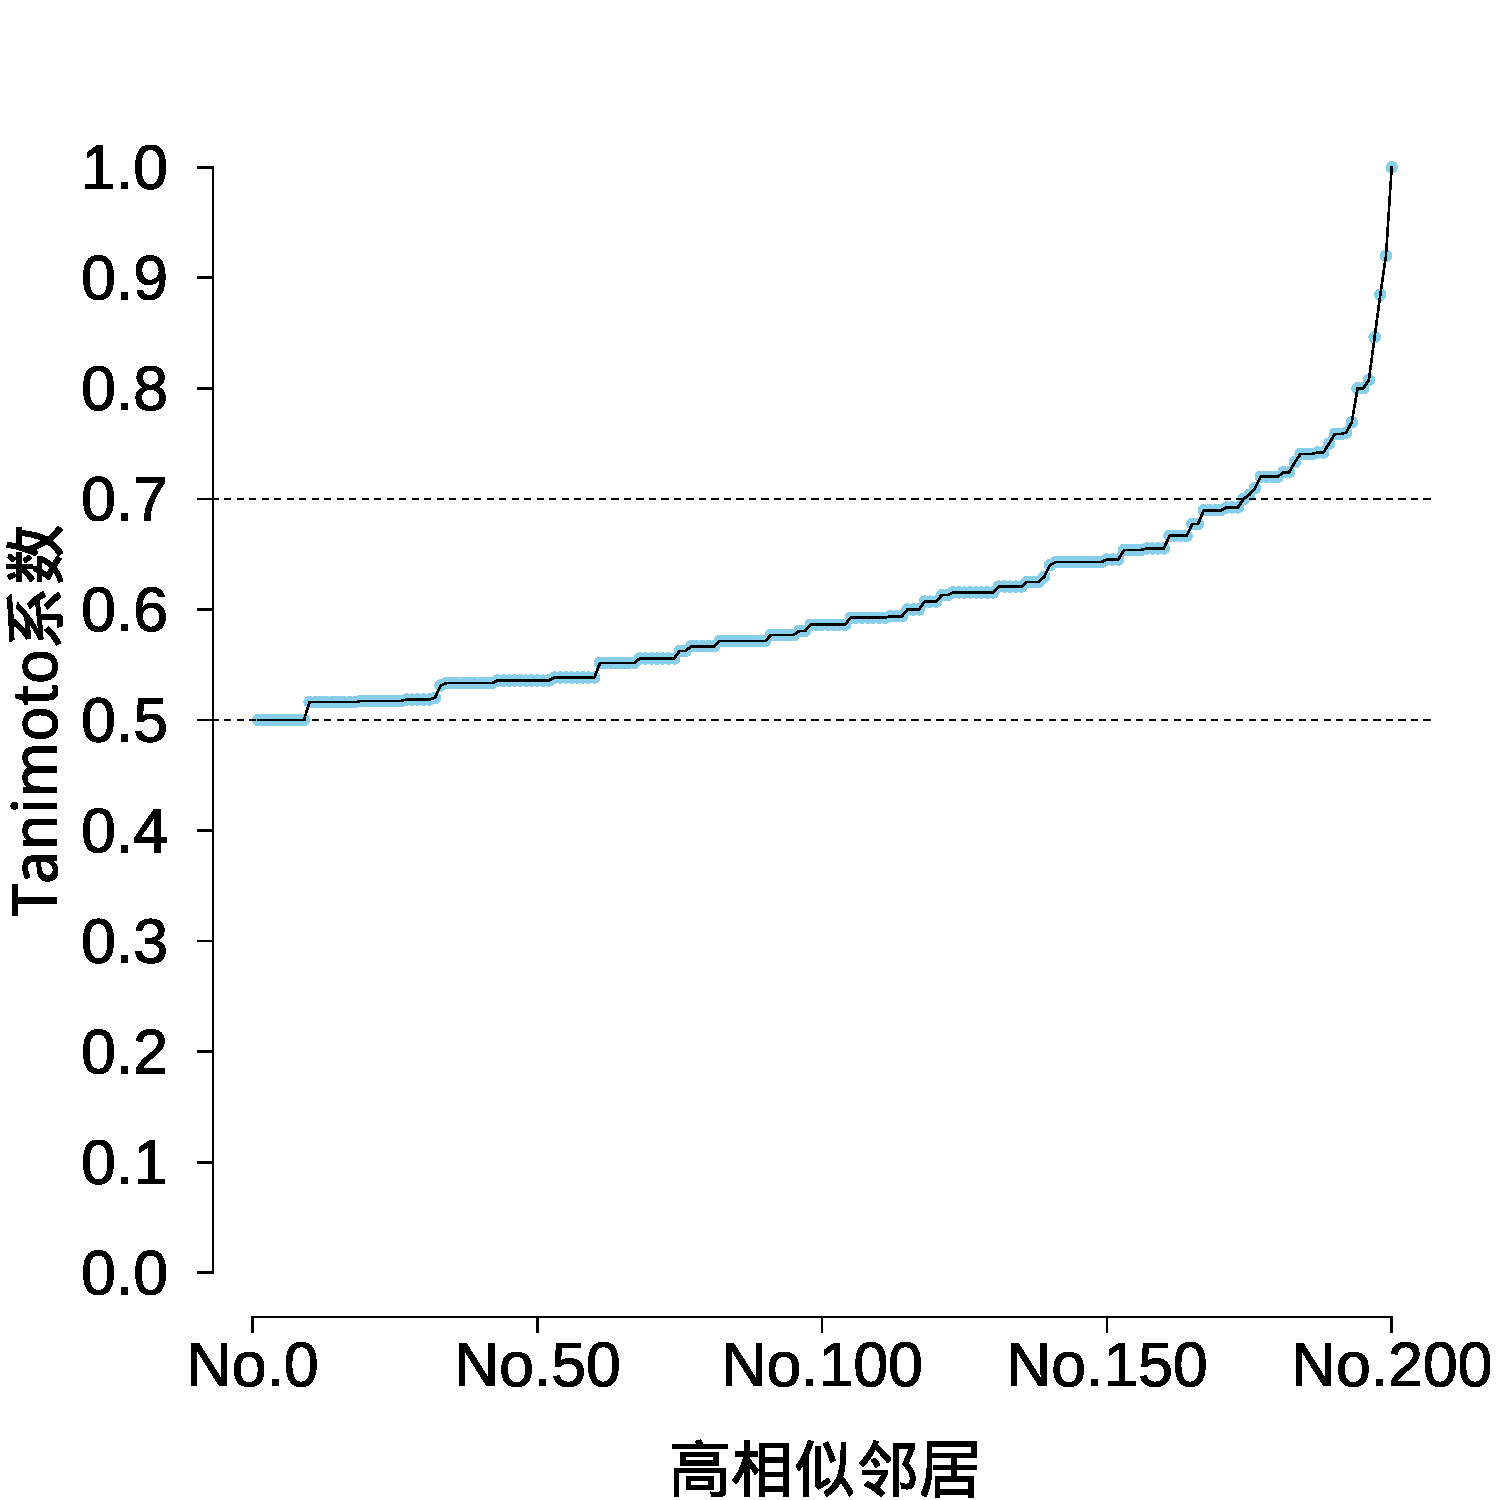
\includegraphics[width=0.5\textwidth]{figures/n_exp.pdf}
\caption{药物组合'Vinblastine sulfate', 'Melphalan'的\\高相似邻居Tanimoto系数图\label{fig:nco}}
\end{figure}

通过对预测结果的观察,在这些药物组合中,可以观察到有一些药物组合的高相似邻居数过多。比如,在NCI-ALMANAC数据集中,有一组药物组合的邻居数最多,它们是'Vinblastine sulfate'和'Melphalan',这组药物组合的邻居数达到了模型求解区间约束的200个邻居。查看它们对应邻居药物组合的Tanimoto系数,从小到大依次排列,如图\ref{fig:nco}所示。可以观察到这200个高相似的邻居中,序号$\mathrm{No.0}$到序号$\mathrm{No.150}$之间药物组合和目标药物组合的Tanimoto相关系数介于0.5到0.7。这表明它们之间具有一定的相关性,但也意味着需要更多相似度更高的药物组合来与目标药物组合匹配,以实现相似的疗效。然而,在实际应用中,这种匹配方法可能会带来问题。治疗方案需要考虑多方面的因素,包括药物之间的相互作用和可能的副作用、患者的个体差异和药物代谢情况等。因此,药物治疗并不可能使用过多的药物组合来治疗病患。如果使用过多的药物组合可能会导致药物相互作用的增加、副作用的加重,并可能会影响药物的疗效。因此,在药物组合治疗中,需要谨慎选择药物组合的数量,以实现最佳的治疗效果。

%插入最少邻居数的图

\section{相关模型的预测结果比较与分析}

本文在横向对比其他模型时,仅采用PCC作为模型的评价指标。这是因为在模型构建前,对数据进行了预处理,这个过程中对原始数据进行了Z-score行标准化,以减少极端值对权重的影响。因此,使用MSE和RMSE等指标进行评估时,DCSN模型与其他使用原始数据的模型相比,结果表现存在超过百倍的差距。在这种情况下,这些指标已失去了比较的价值。因此,本文将重点关注PCC指标来评价模型的表现。

在O'Neil数据集上,本文使用文献\cite{13}中相关的DL模型和ML模型进行比较:深度神经网络(DNN)、梯度提升机(GBM)、随机森林(RF)和支持向量机(SVM),如表\ref{table:model-evaluation}。

\begin{table}[htbp]
  \centering
  \caption{同文献\cite{13}中的模型比较}
  \label{table:model-evaluation}
  \small
  \begin{tabular}{p{4cm}cc}
    \toprule
    Model & PCC & RMSE \\
    \midrule
    DNN & 0.73 & 15.91 \\
    GBM & 0.69 & 16.54 \\
    DCSN & 0.675 & - \\
    RF & 0.65 & 17.49 \\
    SVM & 0.50 & 19.92 \\
    \bottomrule
  \end{tabular}
\end{table}

同时,在NCI-ALMANAC数据集上,本文使用文献\cite{18}中基于高阶分解机(FM)的一阶(comboFM-1)、二阶(comboFM-2),五阶(comboFM-5)模型和随机森林(RF)进行比较,如表\ref{table:sl-evaluation}。

\begin{table}[htbp]
  \centering
  \caption{同文献\cite{18}的模型比较}
  \label{table:sl-evaluation}
  \small
  \begin{tabular}{p{4cm}cc}
    \toprule
    模型 & PCC & RMSE \\
    \midrule
    DCSN & 0.684 & - \\
    comboFM-5 & 0.680 & 62.850 \\
    comboFM-2 & 0.480 & 83.908 \\
    comboFM-1 & -0.156 & 146.672 \\
    RF & 0.41 & 81.27 \\
    \bottomrule
  \end{tabular}
\end{table}

通过比较分析可知,深度学习方法相比于经典机器学习方法,具有更高的PCC,因此具有更优异的效果。而本文所提出的DCSN模型,在PCC方面虽略优于一些机器学习方法,但与深度学习方法相比仍存在较大差距。不过,从实际应用角度考虑,本文的DCSN模型所需的硬件资源较少,最优求解方法仅使用32核CPU运行6个小时即可得出结果。相比较而言,深度学习方法需要依赖显卡进行计算,所需的硬件资源较多,且耗费时间更长。因此,本文所提出的模型具有较低的复杂度,更适合于初期药物筛选阶段的抗癌药物组合协同作用研究,并更利于早期研究的进行。

\section{本章小结}

本章介绍了模型评价与比较的结果。首先,使用PCC和RMSE作为评价指标,评估了四种模型求解方法,发现精细调参法在准确性方面表现最佳,具备强大的泛化能力和预测性能。此外,绘制了协同得分预测值和测试值的散点图,并使用最小二乘回归法对数据进行拟合,结果显示回归系数显著。制作了药物组合邻居数的柱状图和散点图,观察到尽管部分药物组合的高相似邻居选取过多,但大多数药物组合的高相似邻居数较少,具有实际应用意义。最后,对比了其他模型的预测性能,以PCC作为评价指标,尽管与大多数DL模型仍有差距,但DCSN模型的复杂度较低,需要的硬件资源更少,时间成本更低。